\documentclass[11pt]{article}
\usepackage[utf8]{inputenc}  % gebruik de juiste 'character encoding'
\usepackage[dutch]{babel}    % definitie van de taal (Engels is de standaard)
\usepackage{hyperref}        % geef URLs netjes weer
\usepackage{booktabs}		 % mooiere tabellen
\usepackage{a4wide}          % papierformaat en marges
\usepackage{graphicx} 		 % Invoegen van plaatjes , ref: https://nl.sharelatex.com/learn/Inserting_Images
\usepackage{listings}
\usepackage{wrapfig}
\graphicspath{ {images/} }   % zet het pad voor de plaatjes
\pagestyle{plain}            % zet alleen paginanummering aan
% titel en auteur van het document
\title{Onderzoeks verslag DOOMotica}

\begin{document}
	\maketitle % maakt de title
	\begin{figure}[h]
		\centering
		
\includegraphics[width=\textwidth]{inholland}
	\end{figure}
	
	\newpage
	
	\tableofcontents
	\newpage
	\section{Domotica}
	De reden dat we dit project doen is zodat we de domotica in een huis zouden kunnen besturen. Hier voor maken we een webpagina waarop op onder andere de functies van Dahaus, spelletjes, tegeltjes voor je favoriete sites en nog wat andere tegeltjes voor je site geschiedenis.
	\newline
	\newline
	\newline
	\newline
	\section{Website bouwen}
	
	De opdracht voor de studenten is het maken van een website waar de gebruiker een account kan aanmaken en op dit account kan inloggen. Na het inloggen moet de gebruiker zijn favorieten site op de pagina kunnen zetten in de daar aangewezen tegels er voor. verder zijn er nog tegels voor de laatst bezochte sites. verder is er nog plek voor simpele spelletjes en als laatste moet de gebruiker Dahaus kunnen gebruiken.
	
	De web applicatie heeft een aantal eisen:
	\begin{itemize}
		\item Er is een ERD opgesteld voor het Database Management Systeem.
		\item Voor de volgende functies worden PSD's opgesteld:
		\begin{itemize}
			\item Login-functie
			\item Create User-functie
			\item Aanmaken tegels-functie
		\end{itemize}
		\item Door gebruik te maken van XHTML, CSS en ASP.NET wordt de webapplicatie gerealiseerd
	\end{itemize}
	
	\section{Hindernissen}
	
	\subsection{Afwezigheid docent 'Databases'}
	In de afgelopen periode is de leraar voor het vak 'Databases' vier weken afwezig geweest. Dit heeft ervoor gezorgd dat de projectgroep tot week 7 geen les heeft gehad in de onderwerpen: Referentiële integriteit en de vragentaal 'SQL.
	
	De studenten hebben dit geprobeerd op te vangen door zelf onderwerpen te verdelen van het lesplan en zelf uit te zoeken. Voor het assessment zijn alle lessen ingehaald en toegepast op de database. 
	
	\subsection{hashen}
	hashen houd in dat je een wachtwoord zo vervormt met een speciaal algoritme dit kan alleen 1 kant op waardoor het originele wachtwoord niet terug te vinden is. Tenzij je een super computer heb, maar dan ben je nog steeds wel even bezig. Het probleem waar de studenten voor stonden was dat ze hier nog niet eerder mee hadden gewerkt. en dus zelf moesten kijken	hoe het hashen werkt. nadenken te weten hoe het werkt deed hij het nog niet goed, maar na stapsgewijs erdoor heen gelopen te zijn kwamen ze uiteindelijk bij het probleem. Dat na het ophalen van de database de Hash of wachtwoord niet eerst omgezet werd naar bytes. Waardoor de studenten de eerste 16 tekens als salt zagen en wat er na kwam als hash, maar dit hadden de eerste 16 bytes moeten zijn waardoor bij het vergelijken van beide gehashde wachtwoorden niet gelijk waren. Dit hebben De studenten simpel opgelost door het opgehaalde uit de database meteen om te zetten naar bytes.
	
	\subsection{Cookies}
	In de web-applicatie hebben de studenten cookies gebruikt om ervoor te zorgen dat gebruikers ingelogd blijven. Op basis hiervan is ook een Uitlog-knop gebouwd die de cookie moet terugzetten naar de huidige datum -1 dag. Na het drukken op de knop bleef de cookie bestaan en verwijderde de browser deze dus niet. Zie Figuur \ref{Cookie}
	
	In de 9de week(!) kwamen de studenten erachter dat het aan de testbrowser lag. Deze verwijderde de cookies niet wanneer ze waren verlopen, zelfs niet wanneer de gehele browser werd afgesloten. Een oplossing is hiervoor nog niet gevonden.
	
\newpage
	
	\section{Centrale vraag}
	In hoe verre zijn De studenten instaat tot het bouwen van een webpagina. Dit houd in een site met inlog systeem die ook gekoppeld is aan een database en werkende functie heeft zoals Dahaus en spelletjes om te spelen voor de gebruiker. Verder wil de opdrachtgever hoe uitgebreid de studenten de webpagina kunnen maken en wat de studenten nog meer verzinnen om als extra dingen er op te zetten. Denk hierbij bijvoorbeeld aan extra functie als een muziek speler. 
	

	
	\subsubsection{Connectie}
	
	De connectie met DaHaus is gemaakt met behulp van een TCP client. DaHaus is een TCP listener en om met een listener te verbinden moet je een TCP client gebruiken. Er is voor gekozen om de connectie met DaHaus alleen te maken als er een message verstuurd moet worden.
	
	Nadat het bericht is verstuurd wordt de connectie ook meteen weer afgesloten. Het lukte namelijk niet om een connectie te openen en open te houden en op die connectie dan meerdere berichten te sturen en de connectie door middel van een event af te sluiten. Het open houden van de connectie gaf ook het probleem dat als de connectie niet goed werd afgesloten, dan crashde DaHaus. Terwijl nu de connectie automatisch wordt afgesloten waardoor er dus haast geen kans is op een crash van DaHaus.
	\\
	\\
	Om het bericht naar DaHaus te sturen is er een NetworkStream nodig.
	Deze NetworkStream is aangemaakt door via de aangemaakte TCP client een stream te openen. Op deze stream is het mogelijk om een bericht naar plain text te encoden in ASCII en naar DaHaus te sturen in de vorm van Bytes. Als deze bytes zijn verstuurd moet het programma de reactie van DaHaus opvangen. De reactie van DaHaus is ook in plain text en wordt op de zelfde stream terug gestuurd.
	
	Om deze reactie te lezen resetten de webapplicatie de bytes die de studenten gebruikten voor de message, deze worden dan gevuld met wat er van de stream gelezen wordt. Deze bytes worden dan weer terug gezet naar text. Deze text wordt dan in een string gezet en in de response textbox geprint. 
	
	De stream en client worden daarna nog niet gesloten. Eerst wordt de "exit" message naar DaHaus gestuurd. Hierdoor sluit DaHaus de connectie zelf. Daarna wordt de client en de stream geclosed. Deze exit message wordt dan niet geprint, anders komt er na elk commando "Bye bye"\  geprint in de response textbox wat het alleen maar onnodig opvult. De stream en client worden dus pas geclosed nadat DaHaus zelf is ge\"{e}xit. Als de exit message namelijk niet verstuurd werd dan zou de connectie toch nog blijven openstaan bij DaHaus en zou er even goed nog een nieuwe connectie worden gemaakt bij DaHaus bij een nieuwe message. Hierdoor zou er dan een ophoping aan connecties ontstaan bij DaHaus. Dit gaf in kleine tests geen problemen maar bij het opschalen van gebruikers zal het uiteindelijk te veel stress kunnen veroorzaken bij DaHaus. 
	\subsubsection{Commando's}
	
	De commando's die naar DaHaus worden gestuurd kan het best via knoppen worden gedaan. Hierdoor hoeft de gebruiker dan namelijk niet alle commando's uit hun hoofd te kennen of op te zoeken. De makkelijkste optie was om 2 radiobutton lists te maken. \'{E}\'{e}n radiobuttonlist om een object(lamp, window, heater, alle lampen of alle windows) te selecteren. De andere radiobuttonlist zou dan zijn voor de actie die de objecten moeten uitvoeren. Door een lange if else statement te maken is het daarmee mogelijk om voor elke combinatie het bijpassende commando te sturen. Om het commando op te sturen moet de gebruiker dan op de Send button drukken. Als er een ongeldige combinatie wordt gemaakt dan wordt dat in de Response textbox gezet, deze wordt dan niet naar DaHaus gestuurd. De heater wordt van temperatuur veranderd door de Heater en Heater Temp radio buttons te selecteren en in de heater textbox een value te geven. Deze wordt dan gecheckt of het wel een geldig getal is. Als dit getal boven de 35 graden is, dan wordt dit veranderd in 35 graden, dat is namelijk de maximale waarde voor de heater. Zelfde gebeurd met onder de 12 graden, als er een getal onder de 12 ingevuld wordt, dan wordt de heater tot 12 graden gezet. Dat is dus de minimale waarde voor de heater. 
	\subsubsection{Problemen}
	
	Bij de connectie maken met DaHaus zijn veel problemen opgetreden. 
	Er is begonnen bij de commando's op te halen door middel van het "help" commando te sturen naar DaHaus via Putty, op blackboard stond hoe dit gedaan moest worden. Dit zelf leverde geen problemen op. Nu was er toegang tot alle commando's. Daarna moest gekeken worden hoe de connectie met DaHaus gemaakt kon worden. Dit werd gedaan door middel van een TCP client. Deze TCP Client cre\"{e}ren koste tijd om te begrijpen, maar gaf daarnaast geen problemen. Daarna is er uitgezocht hoe de commando's gestuurd konden worden. Dit is geprobeerd op meerdere manieren. Ten eerste werd geprobeerd commando's te sturen door een stream te openen en door middel van handmatig de bytes in de stream te sturen. En daarna de reactie te lezen. Hierbij bleef de stream steken op het lezen van de reactie. Het was niet gelukt om dit probleem op te lossen, er is geprobeerd de volgorde van acties te veranderen, maar verder is er geen informatie gevonden over waarom het niet werkte, er waren namelijk ook geen errors die konden uitleggen waarom de connectie vast liep, omdat dit niet werkte is er naar een andere manier gezocht. Deze manier bestond uit een StreamWriter en StreamReader, alleen hierbij trad hetzelfde probleem op. Daarna is er met behulp van Paul "peregrine" getroubleshoot waarom dit niet werkte. Na het proberen van communicatie tussen eigen gemaakte TCP clients en listeners, bleek dat dat wel werkte. Uiteindelijk is er uitgekomen dat het probleem heel simpel bleek. Er moest namelijk een extra regel in de string van het commando meegestuurd worden.
	\\
	\\
	Het gemaakte programma dat commando's verstuurde was een makkelijk console programma dat na 1 commando meteen de connectie afsloot. Er moest dus nu een webpagina gemaakt worden die dan een beetje gebruiks vriendelijk is. Zoals als eerder al gezegd in het kopje Connectie was er eerst geprobeerd om een connectie te maken en open te houden totdat deze gesloten werd. Dit lukte dus niet.
	
	
	
	
	
	\subsection{Spelletjes}
	De spelletjes die de studenten op de site moeten verwerken zijn simpele spelletjes voor de gebruiker om te spelen op de webpagina zelf. Er kunnen spelletjes op staan zoals: 
	
	
	
	
	\subsection{Tegeltjes}
	De tegeltjes worden in de vorm van een vaste vierkant op de webpagina gepresenteerd. 
	In het opmaakbestand (CSS) wordt de middenkolom in een 'grid' veranderd van minimaal 3 
	kolommen en die worden elk opgevuld met een default plaatje. Op het moment zijn er standaard 9 tegeltjes en deze moeten opgevuld worden met een plaatje en een hyperlink op basis van de ingelogde persoon. (zie Figuur \ref{TegelV1}) \\
		
 	Eerst heeft de projectgroep 9 tegeltjes geplaatst op de Homepagina en deze geprobeerd op te vullen door middel van een 'SELECT'-SQL. Door in de while-loop elke Imagebutton zijn 'ImageUrl'-eigenschap te vervangen door informatie uit de database. Wat hierbij wel verplicht is, is dat de Imagebutton in kwestie dezelfde naam moeten hebben op een cijfer na.\\
 	
 	Als dat lukt dan wil de projectgorep het aantal Tegels aanpassen op basis van de opgeslagen Hyperlinks van de gebruiker. Dus als de gebruiker 5 websites heeft geregistreerd, dat hij/zij dan ook 5 tegels krijgt (zie Figuur \ref{7Tegels} )\\
 	
 	Om tot het eindresultaat te komen heeft de projectgroep een PSD gemaakt, Figuur \ref{PSDTegel}.\\
 	
 	In deze functie wordt op basis van de eerder genoemde 'SELECT'-SQL een button gecreëerd zolang de Datareader nog rijen teruggeeft. Er wordt eerst een imagebutton variabele gemaakt en daaraan worden alle eigenschappen toegevoegd: Een ImageUrl voor het icoon, een hyperlink voor het doorsturen en een omschrijving van de website voor de Tooltip. \\
 	
 	Dan wordt de variabele van de imagebutton toegevoegd aan het grid in de middelste kolom en 
 	onstaat er door het CSS-bestand een net uitziende webdashboard met tegels.
 		
	
	\newpage
	
	\section{Verantwoording gebruikte methodes}
	\subsection{Create user}
	In dit hoofdstuk wordt het aanmaken van een standaard gebruiker besproken. Als een gebruiker zich nog niet heeft aangemeld, dan wordt hij/zij doorverwezen naar de Login pagina. Op deze manier kunnen gebruikers niet zomaar bij elke pagina komen door simpelweg de naam van de pagina in de URL aan te passen. De projectgroep heeft hiervoor een PSD gemaakt (zie Figuur \ref{PSDCU}).\\
	
	
	In de eerste versies van deze functie werd in de Web.config bestanden bijgehouden of er een cookie aanwezig was genaamd "AuthenticationCookie". Tijdens het testen heeft de projectgroep besloten deze functie tijdelijk uit te zetten, omdat zij na elke pauze van 20 minuten werden teruggestuurd naar de Login pagina. Als reactie hierop heeft de projectgroep op elke pagina zelf een functie gezet die controleerd of de "AuthenticationCookie" aanwezig is, en zo niet wordt men terugverwezen naar de login.\\
	
	Tijdens de realisatie is de cookie meer gebruikt dan het web.config bestand voor de beveiliging van de pagina's.	\\
	
	Om ervoor te zorgen dat er één pagina is om naar terug te verwijzen, worden de login en de "Create user" op dezelfde webpagina geplaatst en wordt er gewisseld door middel van buttons.\\
	
	
	Er worden een aantal gegevens van de gebruiker gevraagd, de gebruikersnaam, wachtwoord en e-mail worden gevalideert door een RegularExpressionValidator (regex):
\begin{itemize}
	\item Gebruikersnaam, deze moet uniek zijn en 6-18 tekens bevatten. Regex: 
	\begin{verbatim}
	$(^[A-Z|a-z|0-9|_]{6,18}\$)$
	\end{verbatim}
	
	\item Wachtwoord, 6-15 tekens waarvan 1 hoofdletter en 1 cijfer.Regex:
	\begin{verbatim}
	$(^(?=.*\d)(?=.*[A-Z])(.{6,15})\$)$
	\end{verbatim}
	\item E-mail, deze moet uniek zijn. regex:
	\begin{verbatim}
	$([A-Z|a-z|0-9](\.|_){0,1})+[A-Z|a-z|0-9]\@([A-Z|a-z|0-9])+
	
	((\.){0,1}[A-Z|a-z|0-9]){2}\.[a-z]{2,3}$
	\end{verbatim}
\end{itemize}

Naast de bovenstaande informatie krijgt de gebruiker van het programma een Rolnr, dit nummer geeft aan tot welke pagina's hij/zij toegang heeft. Nu hebben we alles ingevoegd, zie Figuur \ref{Plaintext}.

Het wachtwoord wordt nu nog in plain text opgeslagen en dat is niet veilig. Als volgende stap gaat de projectgroep de wachtwoorden 'hashen'. Dit wordt gedaan in het volgende figuur (Figuur \ref{Hash}). In dit figuur is ook te zien dat in de database een onherkenbare serie letters en cijfers te zien is.

Na het inschrijven van bovenstaande gegevens wordt de gebruiker terug verwezen naar de Login pagina.
	
	\subsection{Inloggen}
	Voor het inlog gedeelte van het systeem zijn de studenten zelf gaan programmeren. Dit omdat de studenten dit een leuke uitdaging leek. Bij het maken van de inlog hebben de studenten een psd gemaakt zoals te zien is in Figuur \ref{Login}. Het Programma is opgebouwd uit een aantal delen deze zijn Het ophalen van het wachtwoord uit de Database. Vervolgens het wachtwoord omzetten naar byte, daarna dan het opsplitsen van de Salt en de Hash. vervolgens de Slat voor het ingevulde wachtwoord zetten. Dit Wordt dan gehashed en als laatst word er vergeleken of de hash van het wachtwoord uit de database en het net gehashde wachtwoord het zelfde zijn, als dit zo is dan word er een cookie gemaakt die de gebruikersnaam onthoud en de gebruiker door stuurt naar de homepage. Wanneer dit niet het geval is krijgt de gebruiker een foutmelding dat het wachtwoord niet correct is. De code is te zien in Figuur \ref{LoginCode}.
	\newpage
	
	\section{Analyse van de gegevens}
	
	\subsection{Dataverzameling}
	De Studenten hebben voor een groot deel gebruik gemaakt van de gegeven powerpoints van de lessen Webprogrammeren. ook hebben we een aantal dingen opgezocht op internet hier de links die we gebruikt hebben: \url{https://msdn.microsoft.com/en-us/library/ms525800(v=vs.90).aspx} (bekeken op \date{19-01-2018}, Geschreven door Microsoft), \newline \url{https://stackoverflow.com/questions/13058574/check-if-cookie-exists}(Bekeken op \date{19-01-2018}, geschreven door zmbq).
	
	\subsection{Analyse}
	De powerpoints waren van een betrouwbare bron. Ze komen namelijk van hun docent die ze les heeft gegeven in webprogrameren en het is ook 1 van de docenten die het project beoordeeld hierdoor weten de studenten ook meteen dat het op de manier gaat als de opdrachtgever wil. De eerste link is afkomstig van Microsoft een betrouwbare bron, omdat het programma waar de studenten hun webpagina op maken ook van Microsoft is. De Tweede links is van de site stackoverflow op deze site stellen mensen vragen over dingen waar ze niet uitkomen met hun programma's. De antwoorden zijn niet altijd betrouwbaar, maar in dit geval werkte het antwoord wel.

	\subsection{Deelconclusie/ aanbeveling}
	De studenten zijn er achtergekomen dat de powerpoints heel handig zijn om bij de hand te hebben voor als je ergens niet op komt. Verder zijn de voorbeelden van Microsoft handig om op te zoeken als je iets niet meer compleet weet. De site stackoverflow is handig als je weet wat je wilt alleen niet weet hoe je het uitvoert. De studenten zouden aanbevelen om zeker de powerpoints te gebruiken en als je het daar niet in kunt vinden kun je altijd nog internet raadplegen. 
	\newpage
	
	\section{Eindconclusie}
	De studenten zijn er achter gekomen dat het meer werk is dan alleen maar een paar dingen op de pagina slepen zoals in de lessen werd gedaan om, maar dat er veel meer bij komt kijken bij een echte webpagina maken met alle eisen zoals beschreven staat in Hoofdstuk 2 staat beschreven. Verder is het handig als zoals bij de studenten gebeurde dat er een les als database uitvalt voor het begin van de periode dat je er zelf gewoon mee aan de slag gaat dan word je achterstand niet te groot.
	
	
	\section{Aanbeveling}
	De aanbeveling van de studenten is om het werk niet te onderschatten en op tijd er mee te beginnen zodat je tijd over kan houden voor extra dingen. Die je op je webpagina wilt zetten. Verder als er een les niet gegeven word om de één of andere reden zoek iemand die er het begrijpt en kan uitleggen en vraag om hulp wanneer nodig, ook aan je groepsgenoten. het is beter hulp te vragen dan het slecht product te leveren.  
	
	\newpage
	
	\section{bijlagen}
	
	\begin{figure}[h]
		\centering
		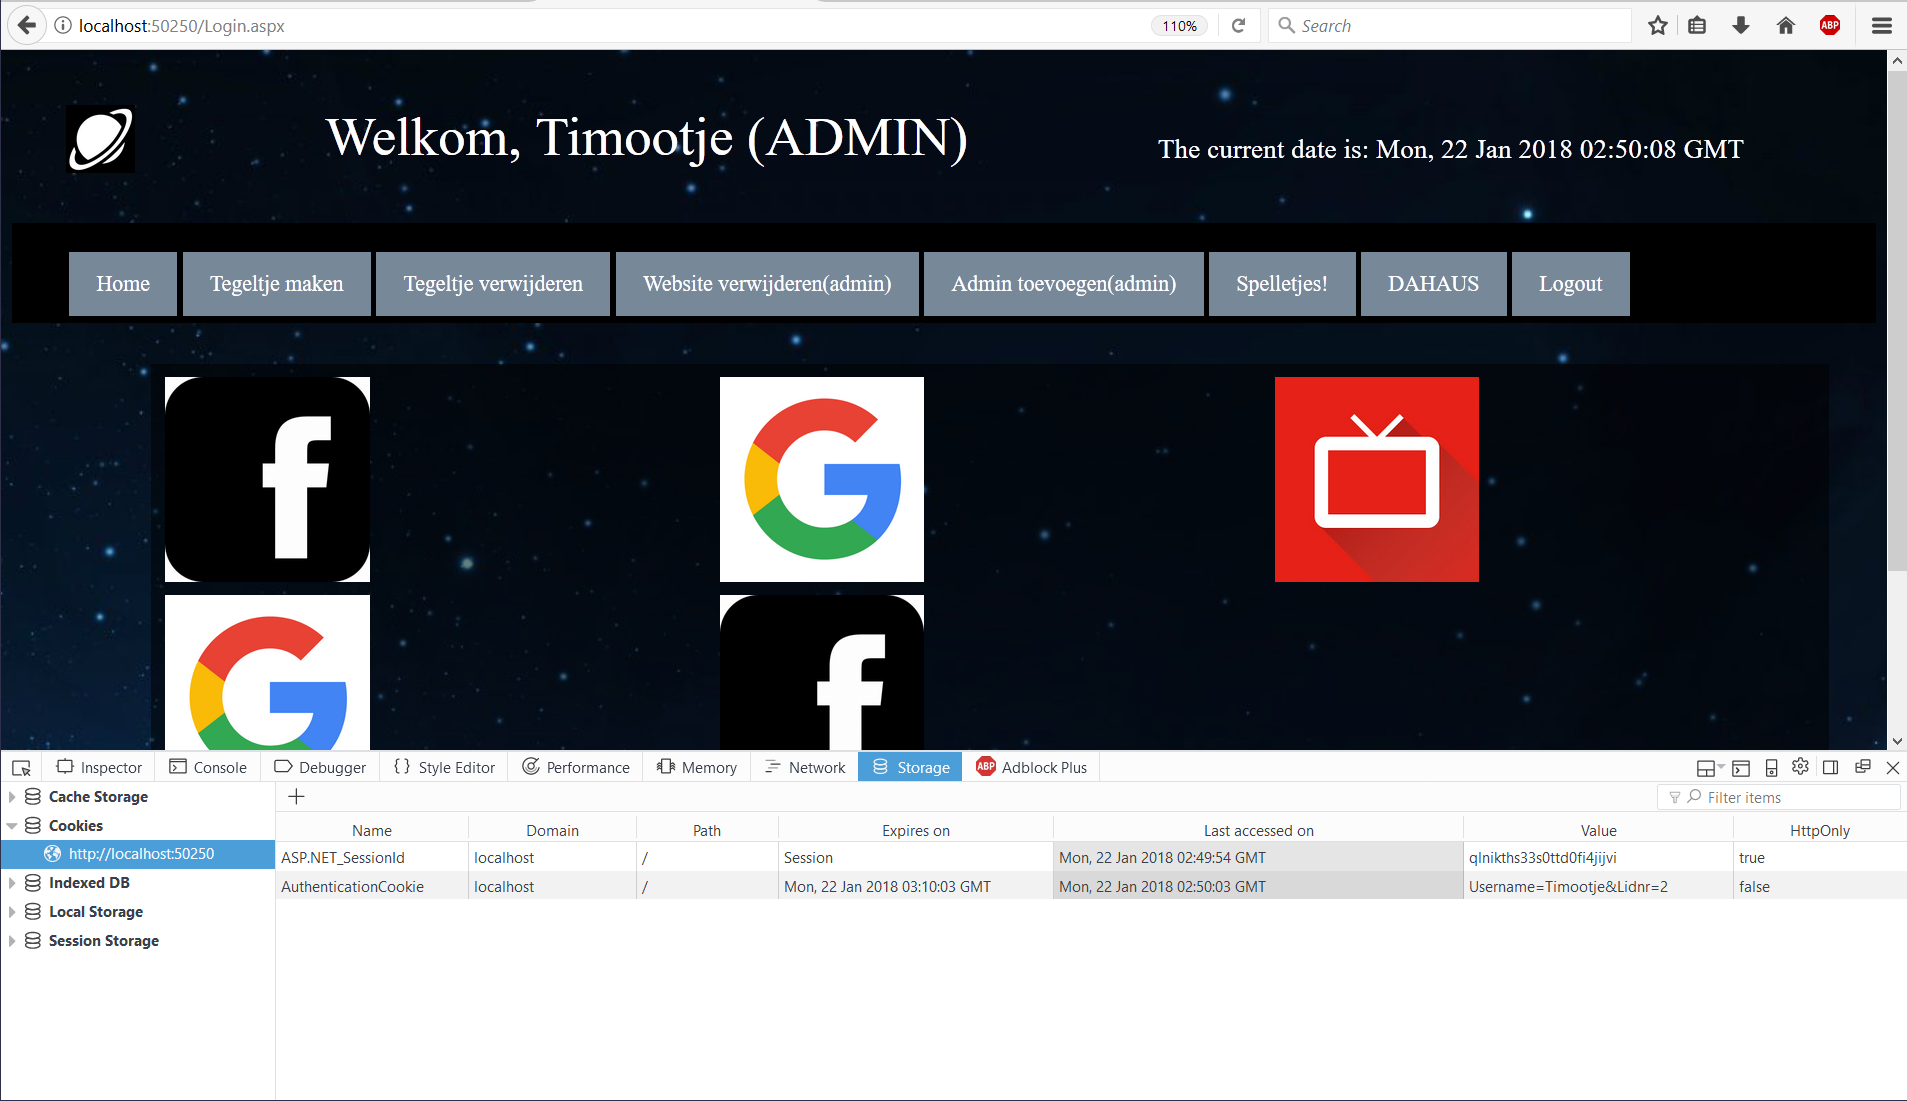
\includegraphics[width=\textwidth]{cookie}
		\caption{De niet verwijderde cookie.}
		\label{Cookie}
	\end{figure}

\newpage
\begin{figure}[h]
	\centering
	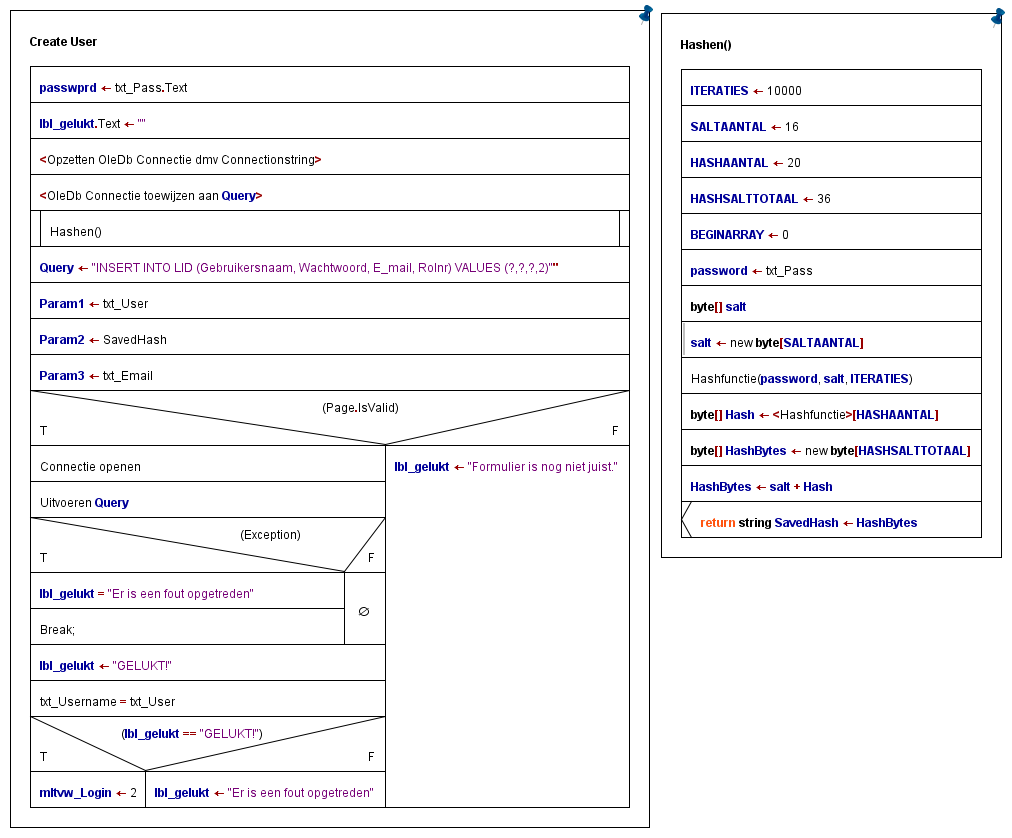
\includegraphics[width=0.7\textwidth]{cu}
	
	\caption{PSD van de functie 'Create\_user'}
	\label{PSDCU}
	
\end{figure}
\newpage
	\begin{figure}[h]
		\centering
		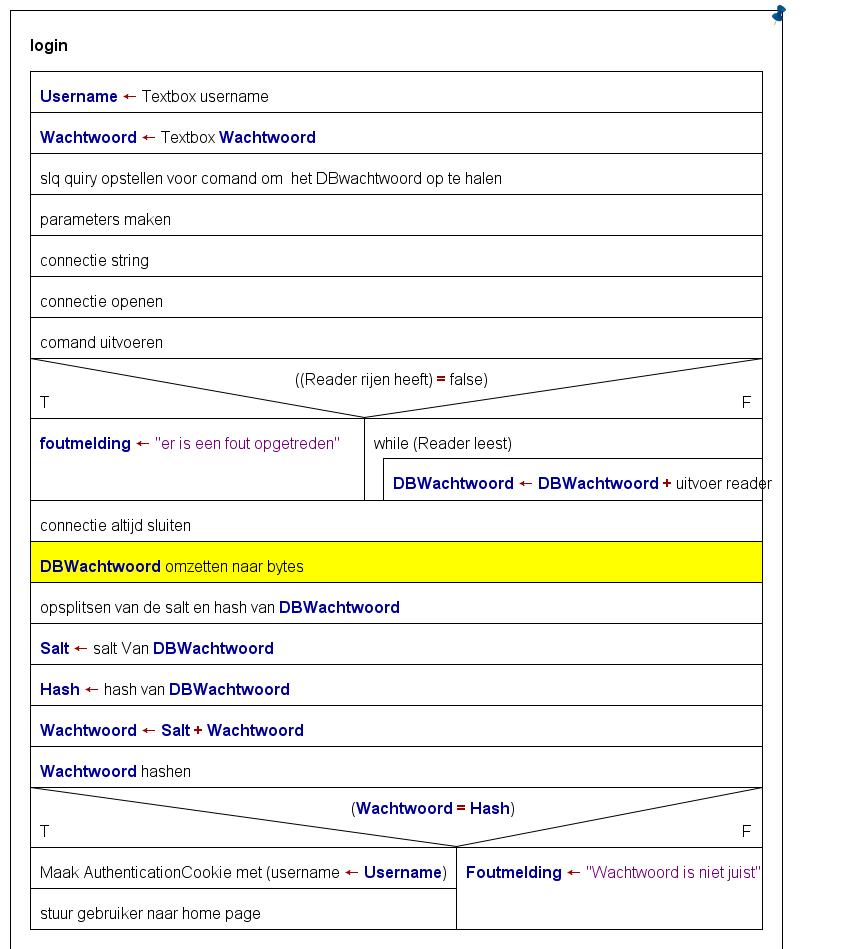
\includegraphics[scale=0.4]{Login}
		\caption{psd van de Login}
		\label{Login}
	\end{figure}
	\newpage
	\begin{figure}[h]
		\centering
		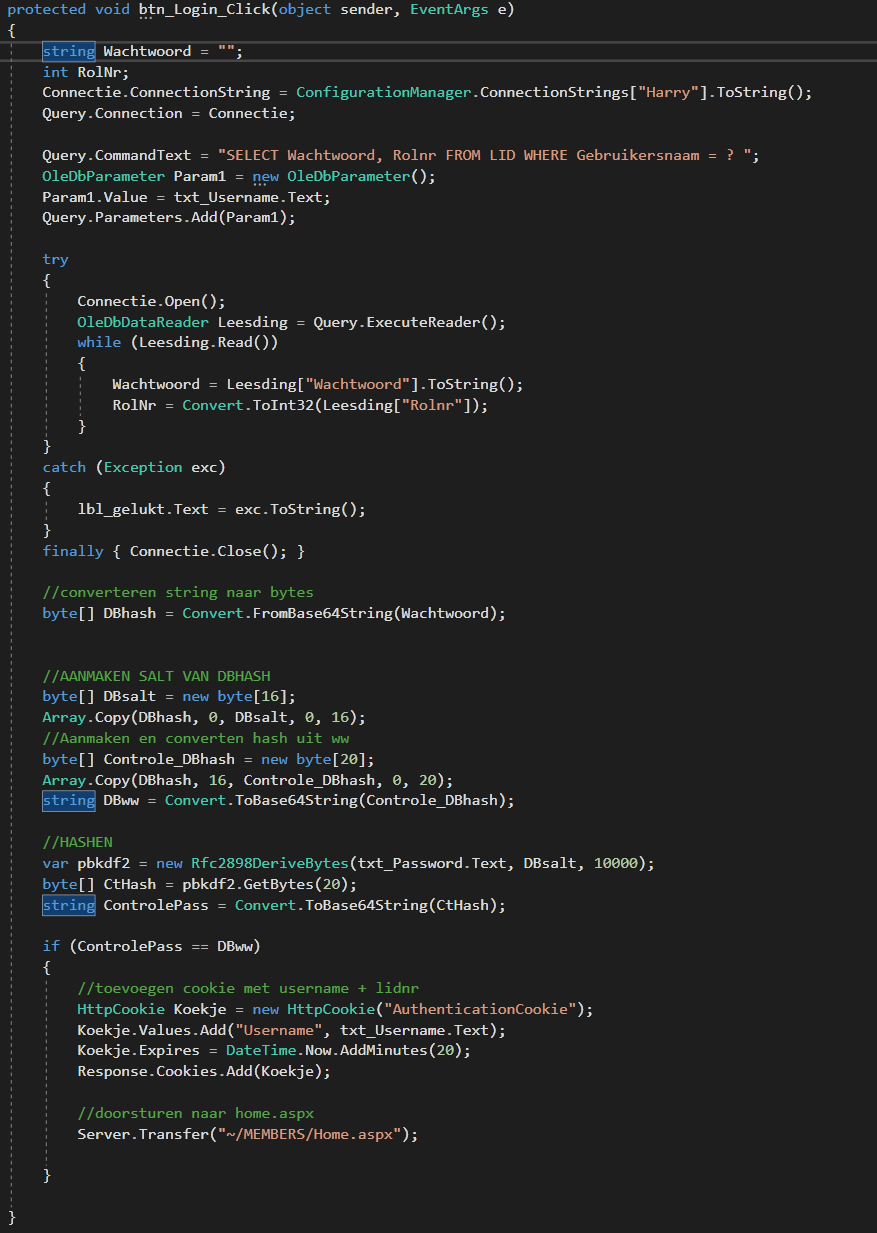
\includegraphics[scale=0.8]{CodeLogin}
		\caption{Code van de login}
		\label{LoginCode}
	\end{figure}
\begin{figure}[h]
	\centering
	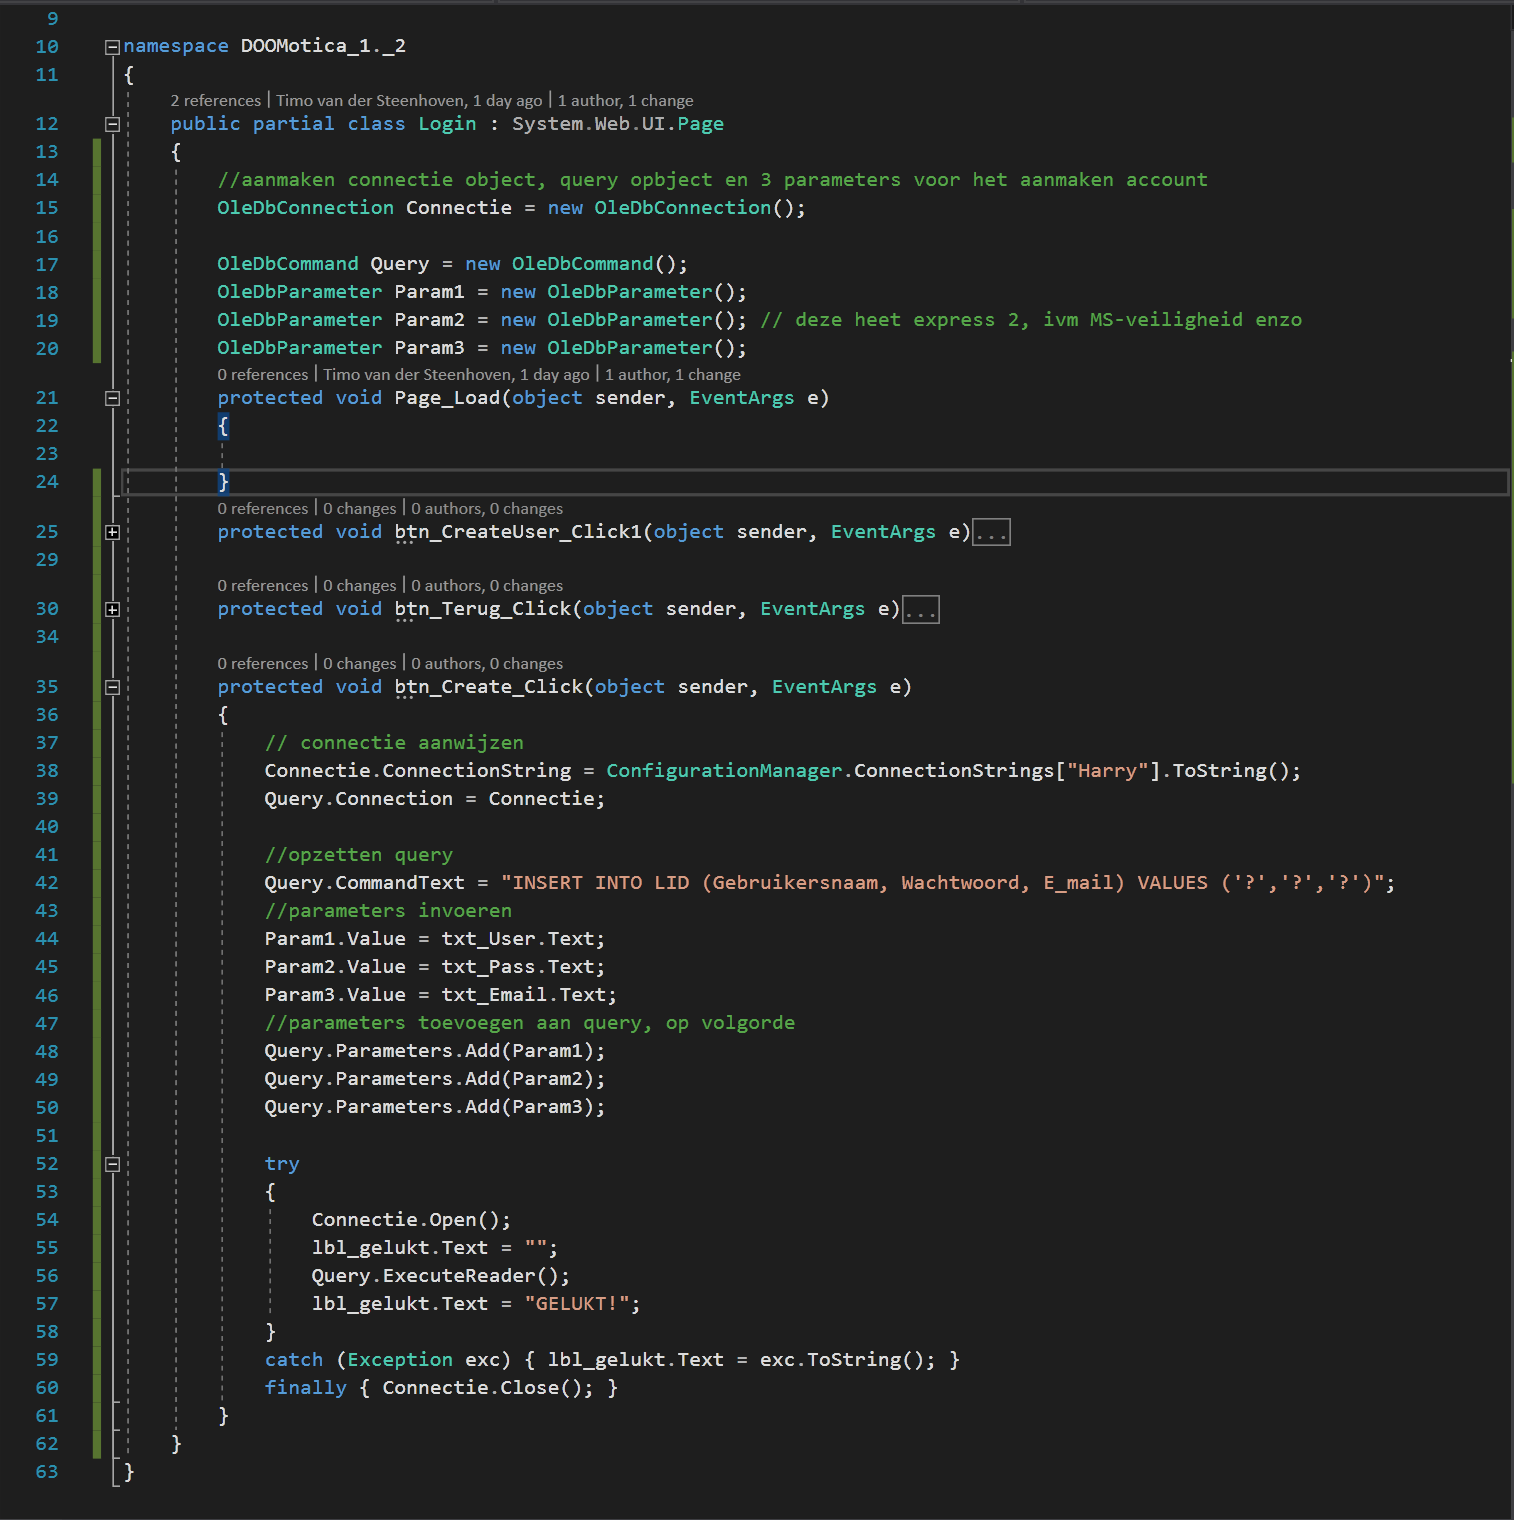
\includegraphics[width=0.8\textwidth]{ipt}
	\newline
	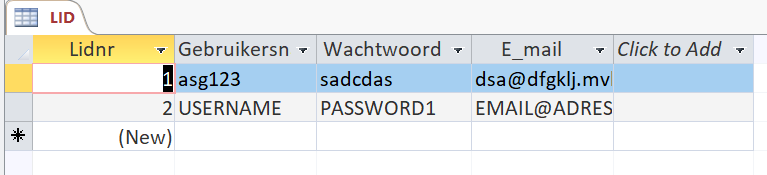
\includegraphics[width=0.5\textwidth]{opt}
	\caption{Opslag plain text en bijbehorende code}
	\label{Plaintext}
\end{figure}
\newpage

\begin{figure}[h]
	\centering
	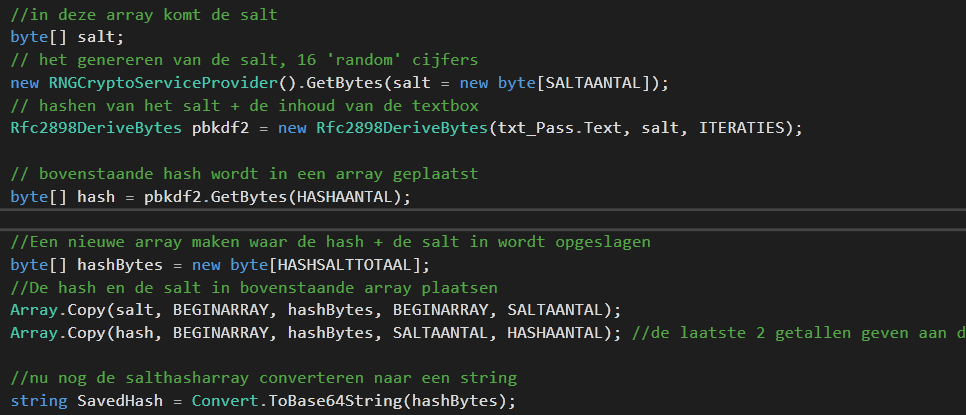
\includegraphics[width=0.6\textwidth]{hash2}
	\newline
	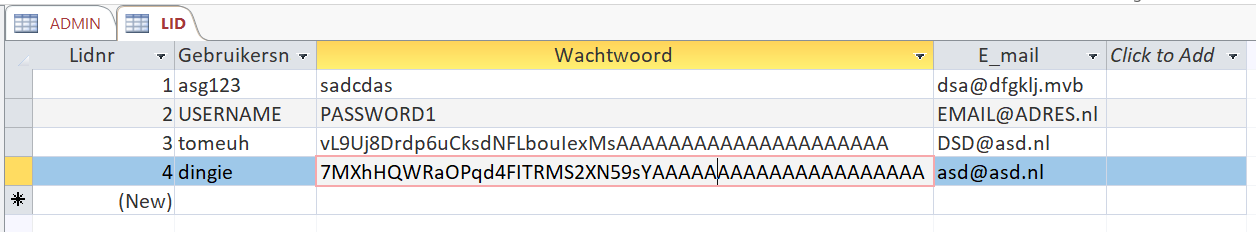
\includegraphics[width=0.5\textwidth]{DTBhashen}
	\caption{De code waaruit de hash wordt gegenereerd.}
	\label{Hash}
\end{figure}
	\newpage
	\begin{figure}[h]
		\centering
		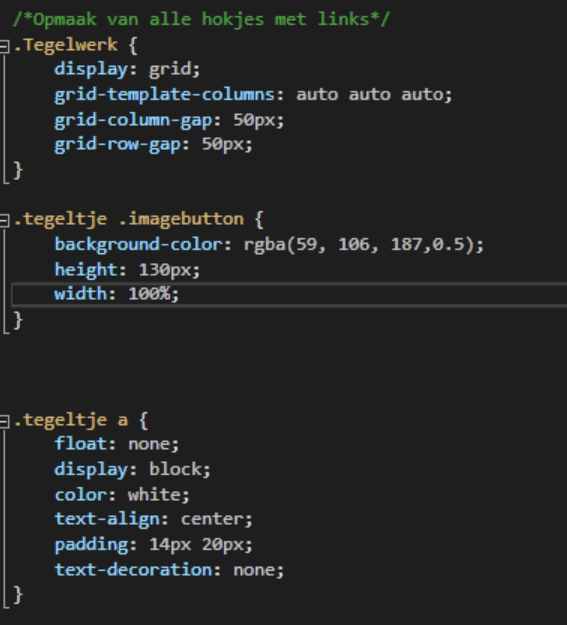
\includegraphics[width=0.5\textwidth]{cssTegel}
		\newline
		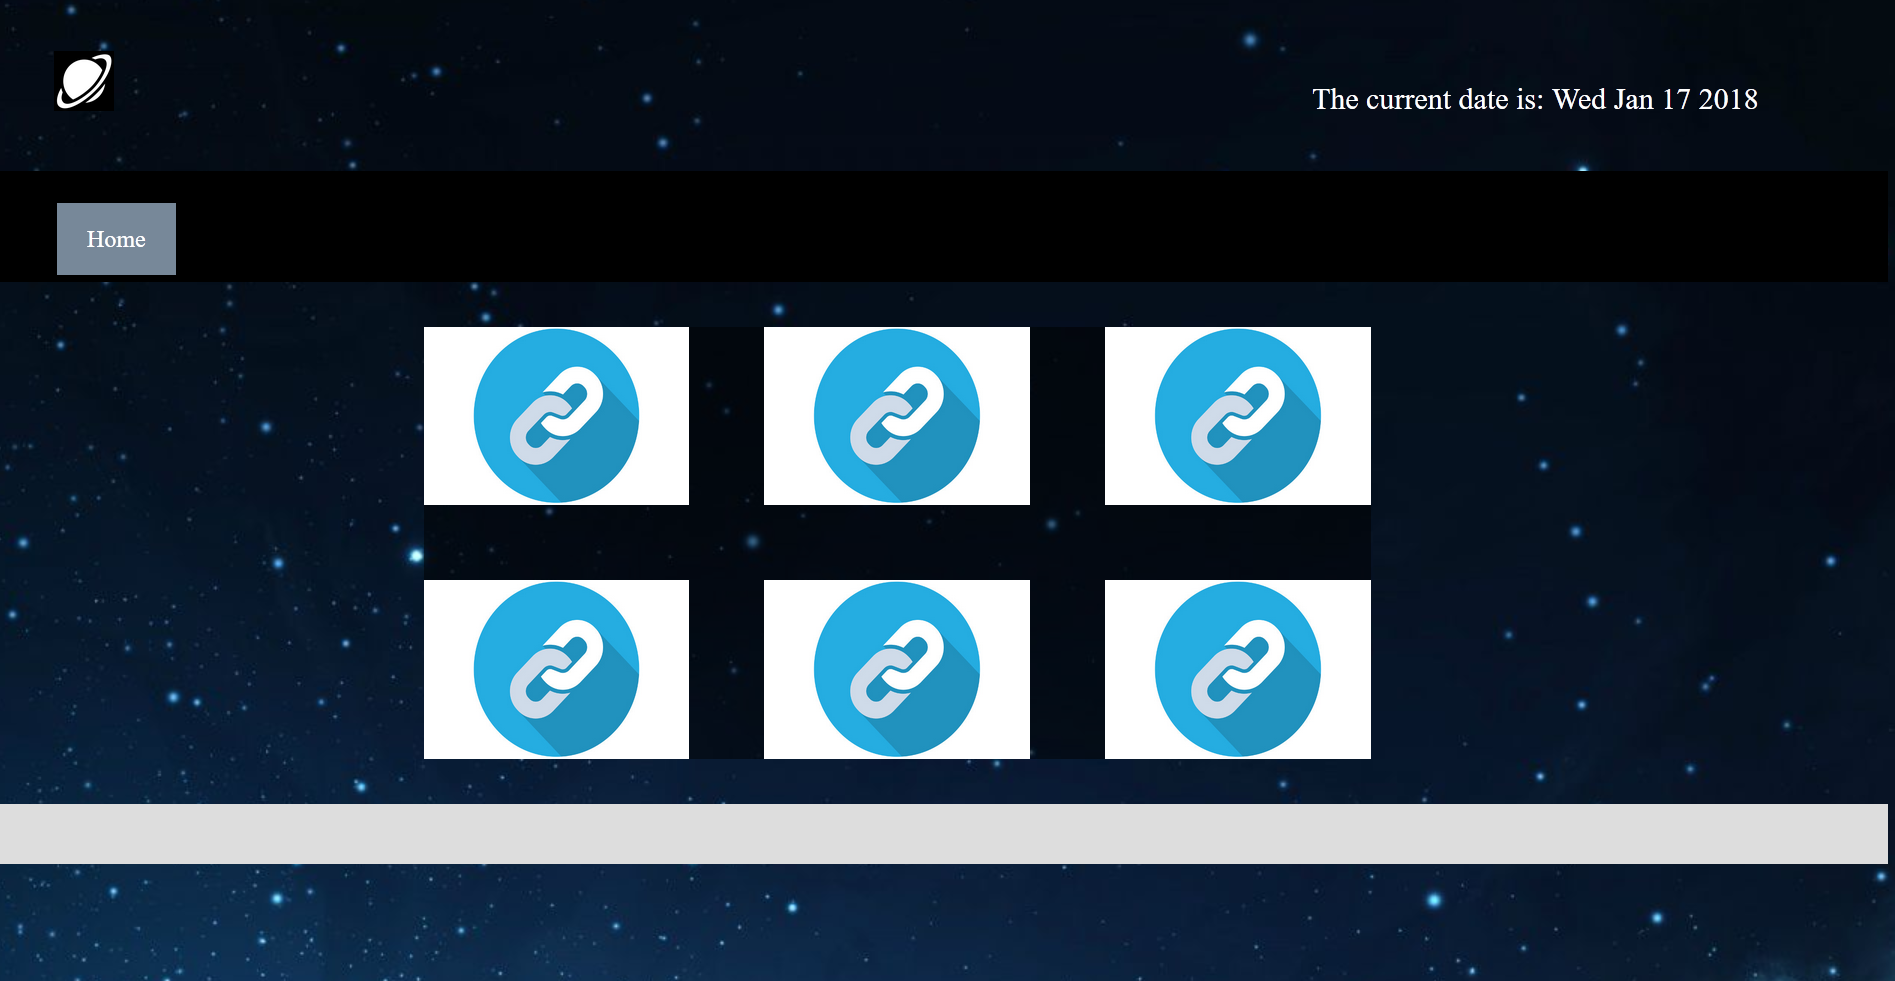
\includegraphics[width=0.7\textwidth]{Tv1}
		\caption{Het resultaat van de CSS opmaak op de tegels.}
		\label{TegelV1}
			
	\end{figure}
\newpage
	\begin{figure}[h]
		\centering
	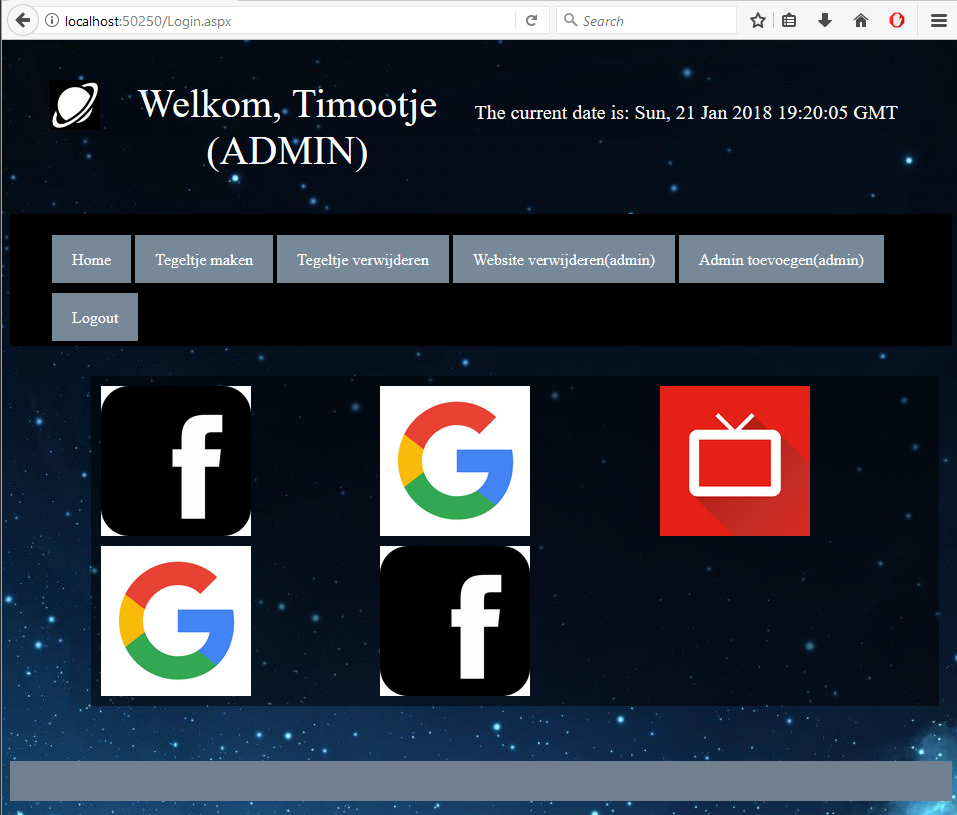
\includegraphics[width=0.7\textwidth]{AdminDelSite3}
	
	\caption{Meerdere persoonlijke tegels}
	\label{7Tegels}
	
\end{figure}
\newpage
	\begin{figure}[h]
	\centering
	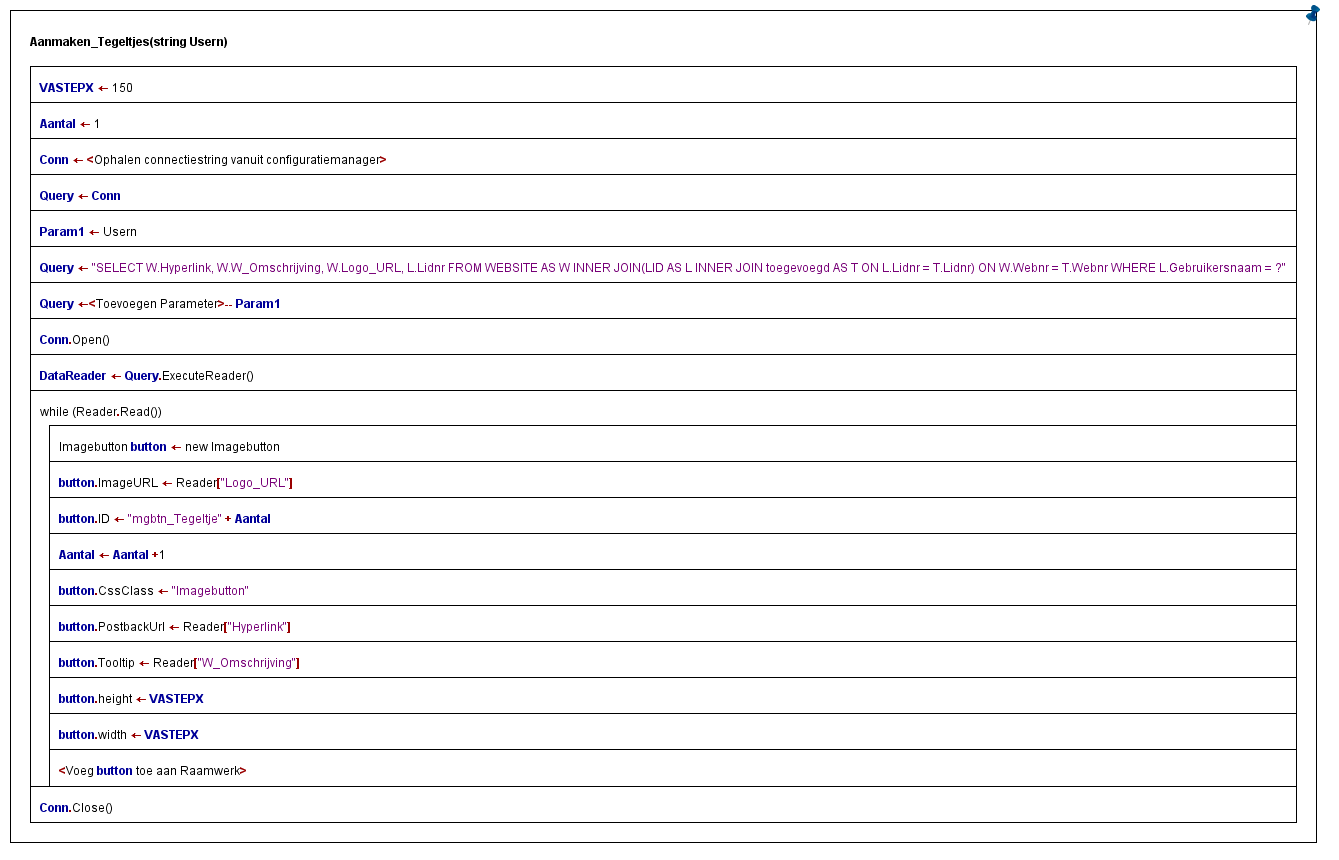
\includegraphics[width=0.7\textwidth]{at}
	
	\caption{PSD van de functie 'Aanmaken\_Tegels'}
	\label{PSDTegel}
	
\end{figure}


	
	
	
	
	
	
	
	
	
	
	
	
	
	
	
	
	
	
	
	
\end{document}